\chapter{Specyfikacja wewnętrzna}
\label{ch:05}

\section{Przedstawienie idei}
\paragraph{}
Widok użytkownika napisany został w języku TypeScript, bazuje na komponentach biblioteki React. Podłoże aplikacji jest oparte na języku Java. Znanym wzorcem projektowym jest MVC (ang. Model View Controller), co przetłumaczone na język polski brzmi: model, widok, kontroler. Model to cześć odpowiadająca za przechowywanie danych. Widok to część dostępna dla użytkownika aplikacji, natomiast kontroler wykonuje operacje i jest odpowiedzialny za logikę programu. Do stworzenia programu wykorzystano architekturę warstwową, która bazuje na MVC oraz skorzystano z wzorca projektowego o nazwie repozytorium. Repozytorium oznacza oddzielenie logiki biznesowej od bazy danych, natomiast architektura wartwowa zakłada istnienie takich warstw jak: encje - będące reprezentacją danych, kontrolery - obsługujące żądania HTTP, serwisy - odpowiedzialne za logikę biznesową i będące wywoływanymi przez kontrolery, repozytoria - mające dostęp do bazy danych, wykonujące operacje zapisu lub pobrania danych. Mapowanie encji na tabele w bazie danych, jak i odwrotnie, jest dostępne dzięki zastosowaniu adnotacji Hibernate.

\section{Opis struktur danych}
\paragraph{}
Dane w kodzie języka Java są reprezentowane przez encje. Są to klasy posiadające pola - zmienne odzwierciedlające kolumny w tabelach w bazie danych. Ich obiekty są odwzorowaniem bazodanowych rekordów. Przykład kodu można zobaczyć na rys. \ref{fig:kod:encja}. Każda zmienna posiada adnotację (poprzedzoną znakiem "@"), jest to składania Hibernate. Dzięki temu jest możliwe mapowanie między obiektem encji, a rekordem w tabeli. Encje posiadają również funckje nazywane getterami - do pozyskiwania danych z konkretnych pól oraz setterami - do wpisywania wartości do pól.

\begin{figure}
\centering
\begin{lstlisting}
@Entity
@Table(name = "user", schema = "adm")
public class UserEntity {
  @Id
  @Column
  private String email;

  @Column
  private String password;

  @OneToMany(mappedBy = "user", fetch = FetchType.LAZY)
  private Set<DriverEntity> driver;

  public String getEmail() {
    return email;
  }

  public void setEmail(String username) {
    this.email = username;
  }

  public String getPassword() {
    return password;
  }

  public void setPassword(String password) {
    this.password = password;
  }

  public Set<DriverEntity> getDriver() {
    return driver;
  }

  public void setDriver(Set<DriverEntity> driver) {
    this.driver = driver;
  }
}
\end{lstlisting}
\caption{Kod encji użytkownika - Java.}
\label{fig:kod:encja}
\end{figure}

\paragraph{}
Aby wysyłać i odbierać dane od tzw. frontendu, czyli części aplikacji dotyczącej interfejsu użytkownika, niezbędne są klasy reprezentujące żądania (ang. request) - odbierane są przez kontrolery oraz odpowiedzi (ang. response) - wysyłane dane do części z językiem TypeScript. Zazwyczaj mają pola analogiczne do encji. Posiadają również funkcje pobierające wartości z konkretynch zmiennych oraz zapisujące wartości do nich, tak jak jest to w przypadku encji. Odpowiedzi są również wyposażone w funkcje konwertujące obiekt encji na obiekt odpowiedzi. Przykład klasy żądania znajduje się na rys. \ref{fig:kod:request}, a metody do konwersji, będącej w klasie odpowiedzi, na rys. \ref{fig:kod:mapper}

\begin{figure}
\centering
\begin{lstlisting}
public class UserRequest {

    @NotNull
    private String email;
    
    @NotNull
    private String password;

    public String getEmail() {
        return email;
    }

    public void setEmail(String email) {
        this.email = email;
    }

    public String getPassword() {
        return password;
    }

    public void setPassword(String password) {
        this.password = password;
    }
}
\end{lstlisting}
\caption{Kod żądania użytkownika.}
\label{fig:kod:request}
\end{figure}

\begin{figure}
\centering
\begin{lstlisting}
public static TrackerResponse fromEntity(TrackerEntity entity){
        TrackerResponse dto = new TrackerResponse();
        dto.setSerialNumber(entity.getSerialNumber());
        dto.setName(entity.getName());
        dto.setType(entity.getType());
        return dto;
    }
\end{lstlisting}
\caption{Funkcja konwertująca encję na odpowiedź.}
\label{fig:kod:mapper}
\end{figure}

\paragraph{}
Analogiczne typy danych zostały stworzone w języku TypeScript w formie interfejsów, pozwalają one w prosty sposób wysyłać żądania i odbierać odpowiedzi. Posiadają one zmienne o identycznych nazwach co klasy w języku Java oraz typy, które pozwalają na automatyczne ich konwertowanie między językami podczas wysyłania i odbierania żądań HTTP. Wygląd interfejsów przedstawia rys. \ref{fig:kod:dto}.

\begin{figure}
\centering
\begin{lstlisting}
export interface UserRequest {
  email: string | null;
  password: string | null;
}
\end{lstlisting}
\caption{Kod żądania użytkownika - TypeScript.}
\label{fig:kod:dto}
\end{figure}

\section{Model danych}
\paragraph{}
Schemat bazy danych znajduje się na rys. \ref{fig:database}. Podstawową tabelą jest tabela użytkownika ("user") - przechowuje ona dane użytkowników systemu. Aplikacja umożliwia dodanie wielu kierowców, pojazdów i lokalizatorów, dlatego tabele: "drivers", "vehicles" oraz "trackers" są powiązane z użytkownikiem relacjami N:1. Dzięki temu jest możliwe wyświetlanie użytkownikowi odpowiednich pozycji w listach, gdyż każdy obiekt jest przypisany do konkretnego użytkownika. Tabela "location" przechowuje dane geograficzne zebrane od urządzeń GPS. Dzięki powiązaniu z tabelą lokalizatorów, można uzyskać łatwy dostęp do historii położenia danego urządzenia. Aby uzyskać dostęp do trasy przebytej przez samochód, niezbędne jest powiązanie między lokalizatorem, a pojazdem reprezentowane przez tabelę "vehicle\_tracker". Analogiczne powiązanie - pojazdu z kierowcą ("vehicle\_driver") - umożłiwia otrzymanie danych lokalizacyjnych dla konkretnego kierowcy.

\begin{figure}
	\centering
	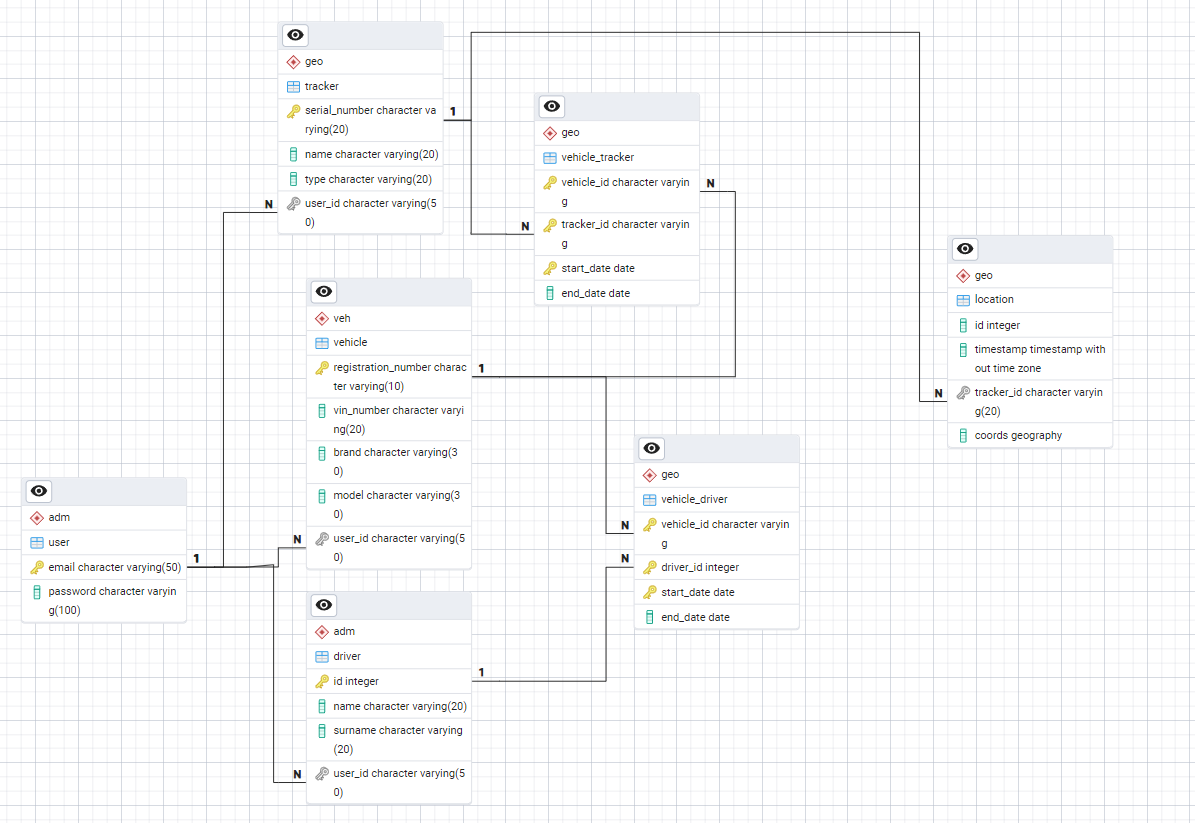
\includegraphics[width=1\textwidth]{./graf/database.png}
	\caption{Schemat bazy danych.}
	\label{fig:database}
\end{figure}

\section{Szczegóły implementacji wybranych fragmentów}

\subsection{Komponenty React}
\paragraph{}
Do stworzenia interfejsu użytkownika wykorzystano komponenty funkcyjne z biblioteki React. Każda zakładka aplikacji posiada oddzielny komponent - każdy w osobnym pliku. Zwracają one JSX, czyli kod zbliżony do HTML, w którym można zagnieżdżać inne elementy. Niemniej jednak, należy pamiętać o zasadzie, iż zwrócić można tylko jeden element nadrzędny - to w nim można umieścić kolejne. Rys.\ref{fig:kod:jsx} pokazuje zwracany JSX przez zakładkę strony głównej (tekst z elementów <p> zostął wycięty).

\begin{figure}
\centering
\begin{lstlisting}
return (
    <div className="main-container">
      <h1 className="welcome-title">Witaj w GeoApp</h1>
      <p className="text description1">
      </p>
      <p className="text description2">
      </p>
    </div>
 );
\end{lstlisting}
\caption{Zwracany JSX przez zakładkę strony głównej.}
\label{fig:kod:jsx}
\end{figure}


Ważnym elementem stworzonej aplikacji są formularze, to dzięki nim użytkownik dodaje obiekty czy powiązania. W tym celu została wykorzystana biblioteka React Hook Form, dostępna w React. Stworzono typy danych, którego przykład można zobaczyć na rys. \ref{fig:kod:formType}. Aby skorzystać z bibblioteki, wykorzystano Hook do destrukturyzacji niezbędnych stałych (rys. \ref{fig:kod:consts}). Aby skorzystać z obsługi formularza, zarejestrowano pola oraz dodano walidacje - przykład na rys. \ref{fig:kod:register}.

\begin{figure}
\centering
\begin{lstlisting}
type FormState = {
  name: string;
  surname: string;
};
\end{lstlisting}
\caption{Typ danych do formularza.}
\label{fig:kod:formType}
\end{figure}

\begin{figure}
\centering
\begin{lstlisting}
const [formState, setFormState] = useState<string>("addDriver");
  const {
    register,
    handleSubmit,
    formState: { errors },
    reset,
  } = useForm<FormState>();
\end{lstlisting}
\caption{Destrukturyzacja stałych z biblioteki React Hook Form.}
\label{fig:kod:consts}
\end{figure}

\begin{figure}
\centering
\begin{lstlisting}
<label className="form-label" htmlFor="name">Imie</label>
<input
  className="form-input"
  id="name"
  {...register("name", { required: "Imie jest wymagane" })}
/>
{errors.name && <p className="form-error form-validation-text">{errors.name.message}</p>}
\end{lstlisting}
\caption{Rejestracja i walidacja pól.}
\label{fig:kod:register}
\end{figure}

Mapa została zaimplementowana przy uzyciu biblioteki Leaflet. Inicjalizacja mapy następuje w useEffect(), czyli w funkcji React, która dzięki pustej tablicy zależności, znajdującej się na samym końcu, wykonuje się raz, gdy komponent mapy zostaje stworzony. Inicjalizację przedstawia rys. \ref{fig:kod:mapInit}. W celu wyświetlania tras na mapie, wykorzystano funkcję polyline(), która łączy linią kolejne punkty, przekazane jako argument w formie tablicy. Ta część kodu widnieje na rys. \ref{fig:kod:polyline}. Utworzona trasa zostaje dodana do mapy. 

\begin{figure}
\centering
\begin{lstlisting}
useEffect(() => {
    if (!mapRef.current && document.getElementById("map")) {
      mapRef.current = leaflet.map("map").setView([50.299, 18.787], 13);

      leaflet
        .tileLayer("https://tile.openstreetmap.org/{z}/{x}/{y}.png", {
          maxZoom: 19,
          attribution:
            '&copy; <a href="http://www.openstreetmap.org/copyright">OpenStreetMap</a>',
        })
        .addTo(mapRef.current);
    }
    loadTrackerData();
    loadVehicleData();
    loadDriverData();

    return () => {
      mapRef.current?.remove();
      mapRef.current = null;
    };
  }, []);
\end{lstlisting}
\caption{Inicjalizacja mapy.}
\label{fig:kod:mapInit}
\end{figure}

\begin{figure}
\centering
\begin{lstlisting}
useEffect(() => {
    if (!mapRef.current) return;
  
    mapRef.current.eachLayer((layer) => {
      if (layer instanceof leaflet.Polyline) {
        mapRef.current?.removeLayer(layer);
      }
    });
  
    const latLngs: [number, number][] = locations
      .filter(loc => loc.latitude !== null && loc.longitude !== null)
      .map(loc => [loc.latitude as number, loc.longitude as number]);
  
    if (latLngs.length > 1) {
      leaflet.polyline(latLngs, { color: "blue", weight: 4 }).addTo(mapRef.current!);
    }
  }, [locations]);
\end{lstlisting}
\caption{Dodanie trasy do mapy.}
\label{fig:kod:polyline}
\end{figure}


\subsection{Proces generowania i obsługi żądań}
\paragraph{}
Pierwszym etapem jest wywołanie w komponencie React funkcji wysyłającej żądanie HTTP. Przykładowym procesem będzie pobranie listy kierowców danego użytkownika. Na rys. \ref{fig:kod:startRequest} wywołana zostaje funkcja getDrivers(), której implementację przedstawia rys. \ref{fig:kod:getDrivers}. Jest to funkcja w języku TypeScript, która umożliwia wysłanie żądania z wykorzystaniem metody GET, na bazowy URL z punktem końcowym "/driver". Następnym krokiem jest odebranie żądania w kontolerze, czyli przez część funkcjonalną aplikacji. Implementacja metody kontrolera związana z pobraniem listy kierowców znajduje się na rys. \ref{fig:kod:controlerGetDrivers}. Za logikę jest odpowiedzialny serwis, stąd metoda widniejąca w kontrolerze jest niewielkich rozmiarów. Niemniej jednak, warto zwrócić uwagę na argument o nazwie "auth" - on pobiera dane obecnie zalogowanego użytkownika, które są niezbędne do znalezienia odpowiednich kierowców. Serwis wykorzystuje repozytorium do wyszukania odpowiednich danych z bazy danych - co można zaobserować na rys. \ref{fig:kod:serviceGetDrivers}, a następnie zwraca listę kierowców, która przez kontroler jest wysyłana jako odpowiedź. Ostatecznie te dane trafiają do komponentu React.


\begin{figure}
\centering
\begin{lstlisting}
const loadDriverData = async () => {
    const data = await getDrivers();
    setDrivers(data);
  };
\end{lstlisting}
\caption{Wywołanie funkcji "getDrivers()", wysyłającej żądanie HTTP.}
\label{fig:kod:startRequest}
\end{figure}

\begin{figure}
\centering
\begin{lstlisting}
export async function getDrivers(): Promise<DriverResponse[] | null> {
    try {
        const response = await request("GET", "/driver");
        return response.data;
    } catch (error) {
        console.error("Error getting drivers:", error);
        return null;
    }
}
\end{lstlisting}
\caption{Kod funkcji wysyłającej żądanie HTTP w celu pobrania listy kierowców.}
\label{fig:kod:getDrivers}
\end{figure}

\begin{figure}
\centering
\begin{lstlisting}
@GetMapping("")
public ResponseEntity<DriverResponse[]> getDrivers(Authentication auth) {
     UserResponse user = (UserResponse) auth.getPrincipal();
     return ResponseEntity.ok(driverService.getDrivers(user.getEmail()));
}
\end{lstlisting}
\caption{Metoda kontrolera, pobierająca listę kierowców.}
\label{fig:kod:controlerGetDrivers}
\end{figure}

\begin{figure}
\centering
\begin{lstlisting}
@Transactional
public DriverResponse[] getDrivers(String email) {
    return driverRepository.findAllByUserEmail(email).stream()
            .map(DriverResponse::fromEntity)
            .toArray(DriverResponse[]::new);
}
\end{lstlisting}
\caption{Metoda serwisu, pobierająca listę kierowców.}
\label{fig:kod:serviceGetDrivers}
\end{figure}